\subsection{Problem Domain}
In this subsection we analyse the the problem domain using the object oriented methods. The problem domain looks at how a bus system currently works.

\subsubsection{Event Table}

Bellow is an event table that what made. It contains the classes and events of the problem domain. It was made to help figure what events the different classes are using.

\begin{table}[H]
\centering
\label{event-table}
\resizebox{\columnwidth}{!}{%
\begin{tabular}{|l|l|l|l|l|l|l|l|}
\hline
\diagbox{\shortstack{Events}}{Classes}& Passenger & Potential Passenger & Ticket & Bus Driver & Bus Stop & Bus Controller & Bus \\ \hline
Open/close door            &           &                     &        & x          &          & x              & x   \\ \hline
Push stop button           & x         &                     &        & x          &          & x              &     \\ \hline
See Potential Passengers   &           &                     &        & x          &          &                &     \\ \hline
Detecting obstacles        &           &                     &        & x          &          &                &     \\ \hline
Halt at bus stop           &           &                     &        & x          & x        &                & x   \\ \hline
Buy/print ticket           & x         &                     & x      & x          &          & x              &     \\ \hline
Start Bus                  &           &                     &        & x          &          & x              & x   \\ \hline
Turn bus off               &           &                     &        & x          &          & x              & x   \\ \hline
Person steps on            & x         & x                   &        &            &          &                & x   \\ \hline
Person steps off           & x         & x                   &        &            &          &                & x   \\ \hline
Maneuver the bus           &           &                     &        & x          &          & x              & x   \\ \hline
Safety handling            &           &                     &        & x          &          & x              & x   \\ \hline
Person arrives at bus stop &           & x                   &        &            & x        &                &     \\ \hline
Person leaves bus stop     &           & x                   &        &            & x        &                &     \\ \hline
Invalid ticket             &           &                     & x      & x          &          & x              &     \\ \hline
Start shift                &           &                     &        & x          &          &                &     \\ \hline
End shift                  &           &                     &        & x          &          &                &     \\ \hline
Check in                   & x         &                     & x      & x          &          & x              &     \\ \hline
Check out                  & x         &                     & x      & x          &          & x              &     \\ \hline
Starts Leaving Bus Stop            &           &                     &        & x          & x        &                & x   \\ \hline
\end{tabular}%
}
\caption{Event table}
\end{table}

\subsubsection{All Classes and What They Contain}\todo{Text is needed for the classes.}
\begin{itemize}
\item \textbf{Passenger:}

\item \textbf{Potential passenger:}

\item \textbf{Ticket:}

\item \textbf{Bus driver:}

\item \textbf{Bus stop:}

\item \textbf{Bus controller:}

\item \textbf{Bus:}

\end{itemize}


\subsection{Class Diagram for the problem domain}



\begin{figure}[H]
\centering
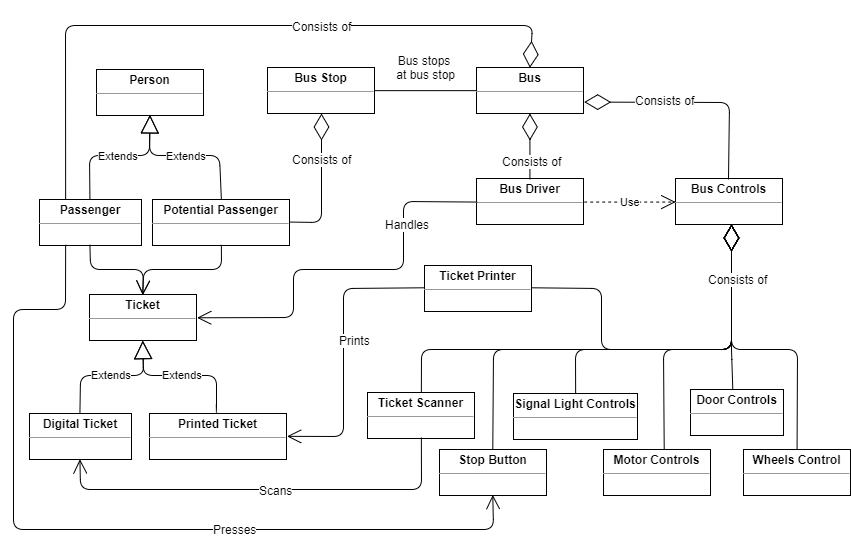
\includegraphics[scale=0.49]{Images/problem_domain_class_diagram.png}
\caption{Class diagram for the problem domain.}
\label{problem-domain-class-diagram}
\end{figure}


\subsection{Behaviour patterns with attributes for each class in the diagram.}

Since the project aim to replace the bus driver

\begin{figure}[H]
\centering
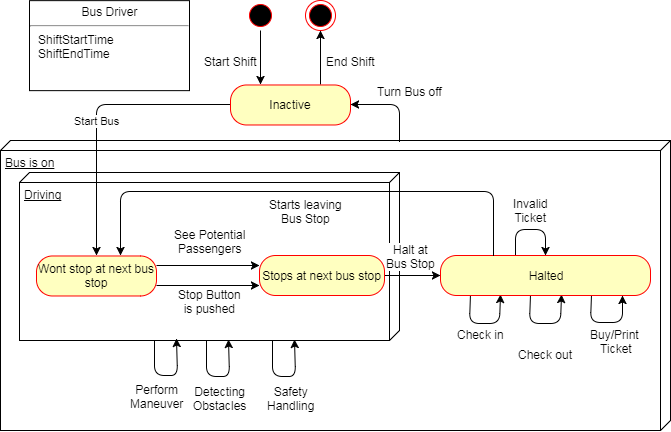
\includegraphics[scale=0.6]{Images/BehaviorDiagramBusDriver.png}
\caption{Behaviour diagram for the bus driver.}
\label{BehaviorDiagramBusDriver}
\end{figure}